\documentclass[11pt]{article}
\usepackage{graphicx}
\usepackage{times}
\textwidth 6.5in
\topmargin 0.0in
\textheight 8.5in
\headheight 0in
\headsep 0in
\oddsidemargin 0in

\title{XORP BGP Routing Daemon \\
\vspace{1ex}
Version 0.3}
\author{ XORP Project					\\
	 International Computer Science Institute	\\
	 Berkeley, CA 94704, USA			\\
	 {\it feedback@xorp.org}
}
\date{June 9, 2003}

%\twocolumn
\begin{document}
\maketitle                            
\section{Introduction}
This document provides an overview of the XORP BGP Routing Daemon.  It
is intended to provide a starting point for software developers
wishing to modify this software.

A router running BGP takes routes from peer routers, filters them,
decides which of the alternative routes is the best, and passes the
winner on to the other peers, possibly applying filters before passing
the route on.

Our chosen architecture for our BGP implementation emphasizes
extensibility and the separable testing of subsystems, rather than
high performance or minimal memory footprint.  However we believe that
the performance and memory usage will be acceptable, even for backbone
router implementations.

We implement BGP as a connected pipeline of ``routing tables'', each
performing a specialized task.  Figure \ref{overview} gives the
general overview of classes involved in the core of the BGP process,
but excludes the classes involved in handling peerings with peers.
\begin{figure}[htb]
\centerline{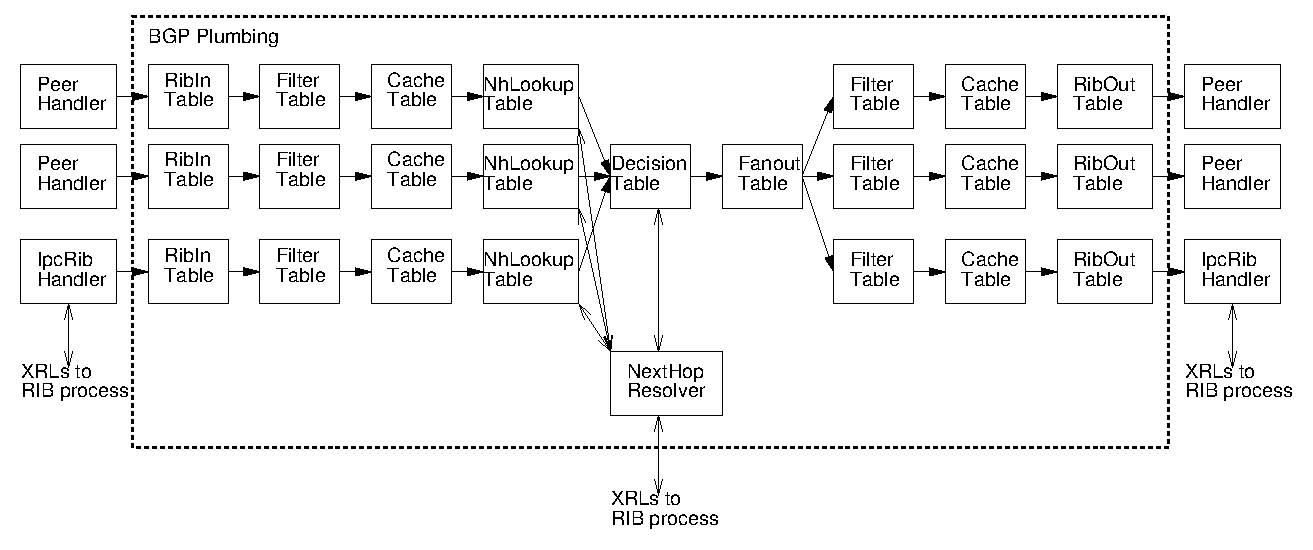
\includegraphics[width=1.0\textwidth]{figs/overview}}
\vspace{.05in}
\caption{\label{overview}Overview of BGP process}
\end{figure}
Route information flows from left to right in this figure.  Typically
an Update or Withdraw message arrives from a BGP peer, is split up
into separate {\tt add\_route} or {\tt delete\_route} commands by the PeerHandler,
and then the update flows through the tables towards the
DecisionTable.  If the route is better than the best alternative, then
it passes through the DecisionTable, and is then fanned out to all the
output branches except the one it arrived un.  The outgoing
PeerHandler then sends the route on to the corresponding BGP peer.

There is one input branch and one corresponding output branch for each
BGP peer, plus one branch that handles routes sent to BGP from the
XORP RIB, and sends BGP routes to the XORP RIB and hence on to the
forwarding engine.  The general structure of the RIB branch is
identical to that of a peer-related branch, but a special version of
the PeerHandler is used.

\section{Major BGP Classes}
In this section we discuss each of the classes from Figure \ref{overview} in
turn, before discussing how each BGP peer is handled.  Most of these
classes are implemented using C++ templates for the address family, so
they are capable of handling IPv4 and IPv6 in an identical manner.
\subsection{PeerHandler Class}
The PeerHandler acts as the interface between the BGP Peer class
(which handles BGP peering connections) and all the RouteTables that
comprise the BGP plumbing.  A single PeerHandler instance receives 
BGP Update messages coming from the BGP peer and constructs new BGP
Update messages to send to that peer.

A BGP Update Message consists of three parts:
\begin{itemize}
\item A list of withdrawn route subnets (route prefixes).
\item Path Attribute information for announced routes.
\item A list of subnets (route prefixes) that are being announced.
The Path Attribute information applies to all these subnets.
\end{itemize}

The PeerHandler splits an incoming update message up, and constructs a
series of messages (InternalMessage class) to send to the plumbing.

Each of the withdrawn route subnets is passed to the plumbing using a
separate {\tt delete\_route} call.

Each of the announced route subnets is passed to the plumbing using a
separate {\tt add\_route} call, which includes all the Path Attribute
information.

On the output side, the PeerHandler receives a series of {\tt add\_route},
{\tt delete\_route}, or \\
{\tt replace\_route} calls.  Each batch of calls is for
routes that share the same path attribute list.  The PeerHandler then
constructs an Update Message from each batch, and passes it on to the
classes that handle the peering for transmission to the relevant BGP
peer router. 

In some cases the PeerHandler can receive routes from BGP faster than
the connection to the relevant peer can handle them.  The PeerHandler
can communicate this information back upstream to regulate the flow of
changes to a rate that can be accommodated.  The actual queuing then
happens upstream in the FanoutTable.

Because of the way BGP encodes IPv6 routes, the PeerHandler class
handles IPv4 and IPv6 routing information differently.

\subsection{RibInTable Class}

The RibInTable class is responsible for receiving routes from the
PeerHandler and storing them.  These are the raw routes, unfiltered
and unmodified except for syntactic correctness, as received and
decoded from the BGP Peering session.

Because BGP does not indicate in an Update message whether a route is
new or merely replaces an existing route, all routes are checked to
see if they are already stored in the RibIn.  If so, the {\tt add\_route} is
propagated downstream as a {\tt replace\_route}, otherwise it is propagated
as an {\tt add\_route}.

The RibIn serves several additional purposes:
\begin{itemize}
\item It can answer {\tt lookup\_route} requests from downstream.
\item When a new peer comes up, a route dump is initiated so that the
new peer learns all the feasible routes that we know.  The RibIn can
perform this dump as part of a background task, so as to allow further
updates while the dump is taking place.
\item When the peer associated with the RibIn goes down, a process to
delete all the routes learned from this peer is started.  This is done
by transferring the RibIn's entire routing table to a new RouteTable
called a DeletionTable that is plumbed in directly after the RibIn.
The DeletionTable handles the deletion of the routes as a background
task, leaving the RibIn ready to cope immediately if the peer comes
back up again.
\item When the routing information in the XORP RIB changes, the change
of IGP metric can change which routes should win the decision process.
The RibIn can be told that the routing information associated with the
indirect nexthop in a BGP route has changed, and it can initiate a
background task that re-sends all the relevant routes downstream as
{\tt replace\_route} messages, so that the DecisionTable can make its choice
again.
\end{itemize}

The RibIn does not do significant sanity checking on its inputs - it
is the responsibility of the receive code in the Peer classes to check
that received update messages are syntactically and semantically
valid.

The current (Mar 2003) version of XORP stores all routes in the RibIn,
irrespective of whether or not they will fail to pass a downstream
filter.  However, the RibIn has enough information (from the values
returned by the {\tt add\_route}, {\tt delete\_route} and {\tt
replace\_route} calls it makes downstream) to be able to store only
those routes that will not be filtered.

\subsection{FilterTable Class}

The FilterTable class has one parent (upstream) RouteTable and one
child (downstream) RouteTable.  It acts as a general purpose
filter-bank, passing, modifying, or dropping routing information that
travels from parent to child.

A FilterTable can hold many filters.  Current filters include:
\begin{itemize}
\item {\bf SimpleASFilter:}  Drops routes that contain the configured
AS in their AS Path.
\item {\bf ASPrependFilter:} Prepends the configured AS number to the
AS Path of all
routes that pass through the filter.
\item {\bf NexthopRewriteFilter:} Changes the NextHop attribute of all
routes that pass through the filter to the specified value.
\item {\bf IBGPLoopFilter:} Drops all routes that we heard through
IBGP.  This is primarily useful as an outbound filter to an IBGP peer.
\item {\bf LocalPrefInsertionFilter:} Inserts the configured value as
the BGP Local Preference attribute in all routes that pass through the
filter.  Typically used on input from an EBGP peer, before
route-specific filters.
\item {\bf LocalPrefRemovalFilter:} Removes the BGP Local Preference
attribute from all routes that pass through the filter.  Typically
used on output to an EBGP peer.
\item {\bf MEDInsertionFilter:} Adds a Multi-exit Descriminator
attribute based on the routes IGP metric to each route that passes
through the filter.  Typically used on output to an EBGP peer.  Note
that the MED to be inserted will have been added to the route by the
DecisionTable, so MEDInsertionFilter cannot be used as an input-branch
filter.
\item {\bf MEDRemovalFilter:} Removes the  Multi-exit Descriminator
attribute from all routes that pass through the filter.  Typically
used just before a MEDInsertionFilter to remove the MED received from
the previous AS.
\end{itemize}
Note that filters are not just for operator configured filtering -
they comprise part of the basic BGP processing mechanism.

Typically a FilterTable will receive an InternalMessage from its
parent containing a subnet route.  All the configured filters will be
applied in order to the route.  One of three things may happen:
\begin{itemize}
\item The route may be dropped by a filter.
\item The route may pass through all filters unchanged.
\item One or more filters may modify the route.  This is done by
creating a new copy of the route.
\end{itemize}
In the last case, the modified route will have the Changed flag set
before it is propagated downstream.  This flag indicates that no-one
upstream is storing a persistent copy of this route, so the downstream
tables are responsible for either storing the route or freeing the
memory it uses.

Filter implementors should be careful to note that if the route
received as input to a filter is already modified, and their filter
then drops the route or creates a modified copy of the route, then the
old route MUST be freed because no-one else can do so.  If the input
route is not modified, the filter MUST NOT free the route because it
is stored elsewhere.

\subsection{CacheTable Class}

The CacheTable class has one parent RouteTable and one child
RouteTable.  Its purpose is to ensure that routes changed by preceding
filter-banks are actually stored somewhere.  Primarily it is an
optimization to prevent the filters from having to be applied every
time {\tt lookup\_route} is called, but it also simplifies memory management
because downstream tables no longer need to be concerned with whether
a route needs to be freed or not. 

The CacheTable takes as input InternalMessages from its parent, and
passes them through downstream to its child.  If the route in the
message does not have the Changed flag set, then the CacheTable is a
no-op.  If the route in the message has the Changed flag set, then the
CacheTable will store the route (or delete it from storage in the case
of {\tt delete\_route}).  Thus all InputMessages sent downstream have the
Changed flag cleared.

A CacheTable in the outgoing branch is flushed (all stored routes
deleted) when the peering corresponding to the relevant plumbing
branch down.  This is because when the peering comes back up, the
outgoing branch should restart with no stored state.  The incoming
branch CacheTable is not explicitly flushed, because the routes will
be removed as the DeletionTable gets round to deleting them.
Prematurely flushing the input branch CacheTables would potentially
result in the DecisionTable seeing inconsistent inputs.

Note that assertion failures in the CacheTable usually indicate that
the code upstream is incorrectly propagating changes (for example
either a delete with no add, two deletes, or two adds).

\subsection{NhLookupTable Class}

The BGP decision process implemented in DecisionTable is relatively
complex, and takes into account many possible factors including ``IGP
distance''.  IGP distance is the IGP routing metric for the route to
reach the BGP NextHop (which is often a number of IP hops away in the
case of IBGP).  Also of interest is whether the BGP NextHop is
actually reachable according to the IGP protocols.  Because of the
multi-process architecture of XORP, BGP does not know the IGP distance
or whether the nexthop is reachable.  To find out this information,
BGP must query the RIB, and this is done by the NextHopResolver class
instance.  If DecisionTable had to perform this lookup, it would
become very complex because it would have to handle suspending the
decision process while waiting for results from the RIB.  A
multi-threaded implementation would solve this problem, but would
cause other issues.

To solve these problems we insert an NhLookupTable upstream of the
DecisionTable.  NhLookupTable queues any updates with NextHop
information that the NextHopResolver does not know about, pending the
response from the RIB process.  Thus by the time an update reaches the
DecisionTable, the NextHopResolver already has access to the IGP
information related to the BGP NextHop.

A complication comes with {\tt lookup\_route}:
\begin{itemize}
\item if the lookup matches an {\tt add\_route} in the NhLookupTable queue,
the NhLookupTable must return ``lookup unsuccessful''.
\item if the lookup matches a
{\tt replace\_route} entry in the NhLookupTable's queue, the old
answer must be given.
\end{itemize}
In general, the behaviour should be as if the queued updates had not
yet been received from the relevant peer.  Note that the time for the
RIB to respond should normally be very small compared to the usual
delays for propagating Update messages between peers.

\subsection{DecisionTable Class}

The DecisionTable is the core of the BGP process.  It takes route
changes from the input branches, and decides whether those changes are
better or worse than the routes it has already seen.

When DecisionTable receives an {\tt add\_route} from one input branch,
it queries the other peers input branches using {\tt lookup\_route}.
\begin{itemize}
\item If none of the other branches returns an answer, then the route is a
new one, and can be passed on downstream so long as the BGP NextHop is
resolvable.  
\item If one or more of the other branches returns an
answer, one of these answers will have been the previous winner.  The
new route is compared against the previous winner - if it is better
then a {\tt replace\_route} message is propagated downstream.  If it
is worse, then no further action is taken.
\end{itemize}

When DecisionTable receives a {\tt delete\_route} from one input
branch, it queries the other peers' input branches in the same way:
\begin{itemize}
\item If none of the other branches returns an answer, the the {\tt
delete\_route} can be passed on downstream so long as the BGP NextHop
was previously resolvable.
\item If one or more of the other branches returns an
answer, one of these answers will be the new winner.  The routes are
compared, and a {\tt replace\_route} will be sent downstream.
\end{itemize}

The processing for {\tt replace\_route} is similar to that for {\tt
delete\_route} followed by {\tt add\_route}, except that only a single
replace (or delete in the case where the new nexthop is unreachable
and there are no alternatives) will be sent downstream.

\subsection{NextHopResolver Class}

Unlike most of the previous classes, NextHopResolver is not a
RouteTable sub-class.  A BGP implementation has a single NextHopResolver
instance per address family.  The NextHopResolver takes requests to
resolve a BGP NextHop address and attempts to resolve the address to
that of the immediate neighbor router that would be used to forward
packets to the NextHop address.

When it receives an address to resolve, the NextHopResolver first
checks its own routing table.  If the nexthop address can be resolved
there, then the answer can be returned immediately.  Alternatively, if
its own routing table indicates that the address definitely cannot be
resolved, then a negative response can be given immediately.
Otherwise it needs to contact the XORP RIB using XRLs to answer the
question.  

In this way, the NextHopResolver obtains a copy of the relevant subset
of the RIBs database related to the NextHops given by BGP.  The RIB
will also keep track of the subset that it has told BGP about.  If
this information changes in any way BGP will be informed by the RIB,
either directly of the change or that some information is no longer
correct and BGP must query again.

The information held by the NextHopResolver is reference-counted so
that it can be removed when it is no longer relevant.  If the
information contained changes, a notification of the change will be
passed to the DecisionTable, which will propagate the notification
back upstream to the RibIn tables.

\subsection{FanoutTable Class}

The principle task of the FanoutTable is to distribute route changes
that passed the DecisionTable, and therefore are real changes not just
possible changes.  FanoutTable passes a change to all the output
branches except the one where the change originated.  In the case of
{\tt add\_route} or {\tt delete\_route}, this is simple but a {\tt
replace\_route} may contain an old route and a new route that
originate from different peers, so it may be propagated as an {\tt
add\_route} to the peer where the old route originated, as a {\tt
delete\_route} to the peer where the new route originated, and as a
{\tt replace\_route} to all the other peers.

The secondary task of the FanoutTable is to serve as a queuing point
for changes when the BGP peers are not capable of keeping up with
updates at the rate we are propagating them.  The advantage of queuing
updates in the FanoutTable as opposed to in the RibOut or PeerHandler
is that only one copy of the change needs to be kept, no matter how
many peers are not keeping up.  This is particularly important in the
case where the peer from which we heard most of our routes goes down,
and a large number of deletions occur in a short period of time.
These deletions need to go to all the remaining peers, and it is
likely that we can generate them faster than TCP can transfer them to
the peer.

Thus there is a single update queue in the FanoutTable, and a separate
pointer into this queue is maintained for each outgoing branch (and
hence each peer).  If a output branch indicates it is busy, the
FanoutTable will stop propagating changes to it, and instead queue the
changes.  Only when a change has been propagated to all the intended
peers will it be removed from the queue.  

\subsection{RibOutTable Class}

The purpose of the RibOutTable is to communicate changes to the
outgoing PeerHandler and hence on to the relevant BGP peer.  The
RibOutTable class accumulates changes (add, delete or replace) in a
queue, and waits for a flush request.  The reason for the queue is
that the incoming PeerHandler split up a single incoming Update message
into many changes, each with the same Path Attributes.  On output, we
want to accumulate these changes again, so that we can send them on to
our peers in a single Update message.  Thus, after the incoming
PeerHandler has sent the last change to the RibIn, it sends a flush
message through.  When this reaches the RibOut, it is the signal to
take all the changes that have been queued, and build one or more
Update messages from them.  Of course the nature of the decision
process and filters mean that changes that arrived together do not
always result in outgoing changes that share the same Path
Attributes.  Thus multiple passes over the RibOut queue are required,
each accumulating changes that share the same Path Attributes so that
they can be sent on in the same Update message.

In principle, the RibOut could also store pointers to the routing
information that was passed on to the peer so that Route Refresh
(RFC 2918) could be handled efficiently.  In our current implementation
we do not do this - the RibOut maintains no record of the routes
passed to the peer.

\subsection{RibIpcHandler Class}

The RibIpcHandler class is a subclass of PeerHandler, with basically
the same interface as far as communication with the RibIn and RibOut
are concerned. However, instead of communicating with BGP peers, the
RibIpcHandler communicates routes to and from the XORP RIB.  Routes
are received from the RIB if the RIB has been configured to
redistribute routes to BGP.  In addition, all routes we pass to other
peers are also communicated to the XORP RIB, and hence on to the
forwarding engine, so that we can forward packets based on the routing
information.

\section{Background Tasks}

The XORP BGP implementation, like all XORP processes, is
single-threaded.  However, certain simple events can cause BGP to
perform a great deal of work.  For example:
\begin{itemize}
\item When a peering goes down, all the routes in the RibIn associated
with that peer must be deleted, which either results in Withdraws
being sent to all remaining peers, or Updates being sent to indicate
an alternative path is now the winner.  As there can be many thousands
of routes in a RibIn, this process can take some time.
\item When a new peering comes up, all the winning routes must be sent
to that peer.  This can also take some time.
\item When the IGP information related to a BGP nexthop changes, all
the routes that specify this nexthop must be re-evaluated to see if
the change affects the choice of route.  In BGP it is fairly common
for a very large number of routes to share the same BGP nexthop, so
this re-evaluation can take some time.
\end{itemize}
The XORP BGP process cannot simply process such events to completion -
in particular it must keep processing XRL requests from other
processes or the IPC mechanism may declare a failure.  In any event,
it is important that a single slow peer cannot cause route forwarding
between other peers to stall.  Thus we process the events above as
``background tasks''.  

In a multithreaded architecture, such tasks might be separate threads,
but the locking issues soon become very complex.  In our single
threaded architecture, there are no complex locking issues, but the
background nature of such tasks needs to be explicitly coded.  We do
this by dividing the background task into small enough segments.  At
completion of such a segment we schedule a zero-second timer to
schedule execution of the next segment, and drop back to the main
event loop.  Execution will then be restarted after pending network
events and expired timers have been processed by the main event loop.
Care must of course be taken to ensure that when execution returns,
the processing of events or other background tasks has not rendered
incorrect the state the background task needed to restart.  However,
as the processing of each background task segment is naturally atomic
in a single-threaded architecture, there are fewer possibilities for
bad interactions.  Even so, the state stored by these background tasks
to enable their correct restart involves some rather complex
algorithms.

\subsection{DeletionTable Class}

When a peering goes down, the routing table stored in the RibIn is
moved to a DeletionTable that is plumbed in directly after the RibIn,
as shown in figure \ref{del_table}.
\begin{figure}[htb]
\centerline{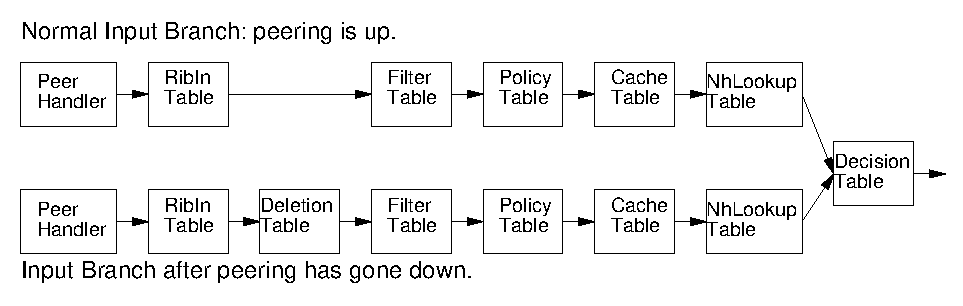
\includegraphics[width=0.7\textwidth]{figs/del_table}}
\vspace{.05in}
\caption{\label{del_table}Dynamic insertion of Deletion Table on
Peering Failure}
\end{figure}
The task of the deletion table is to delete all the routes that were
previously stored in the RibIn, but to do so as a background task
allowing the BGP process to continue to handle new events.

Deletion is scheduled in series of phases.  In a single phase, all the
routes that share a single set of Path Attributes are deleted.  In
this way, if there are alternative routes in a different RibIn that
also share a path attribute list (a fairly common occurrence), then the
chance of preferred route may be batched in such a way that it might be
possible to use a single update message might convey the change to
each neighbor.  At the end of a phase, the DeletionTable schedules
execution of the next deletion phase using a zero-second timer.  This
allows all pending timer or network events to be handled before
deletion resumes.

The DeletionTable must respond to {\tt lookup\_route} requests from
downstream just as a RibIn table would - even though the deletion
table knows the routes it holds will be deleted, it must respond as if
they had not yet been deleted until it has had a chance to send the
relevant {\tt delete\_route} message downstream.  In this way, the
DeletionTable provides a consistent view to the downstream tables - if
they earlier performed a {\tt lookup\_route} and got a specific answer,
then they will still get the same answer unless they have received a
{\tt delete\_route} or {\tt replace\_route} informing them of a
change.

When the last route is deleted from the DeletionTable, the table
unplumbs itself from the BGP plumbing, and deletes itself.

A small complication is added by the possibility that the peering
might come back up before the DeletionTable has finished deleting all
the old routes.  Thus if the DeletionTable receives an {\tt
add\_route} from upstream for a route that in present in the
DeletionTable, then this route would be passed on downstream as a {\tt
replace\_route}, and the route would then immediately be removed from
the DeletionTable.  {\tt add\_route}, {\tt replace\_route} and {\tt
delete\_route} for routes not present in the DeletionTable are simply
passed from parent to child without modification.

Should the peering come up and go down again before all the routes in
the first DeletionTable have been deleted, a second deletion table
would be inserted before the first one.  By virtue of the normal
functioning of the DeletionTable, if there are two such cascaded
DeletionTables, then they will not hold the same route, so this does
not add any additional complication.

\subsection{DumpTable Class}

When a peering comes up, all the currently winning routes from the
other peers must be sent to the new peer.  This process is managed by
an instance of the DumpTable class, which is inserted between the
fanout table and the first table on the output branch to the peer that
came up (see Figure \ref{dump_table}).
\begin{figure}[htb]
\centerline{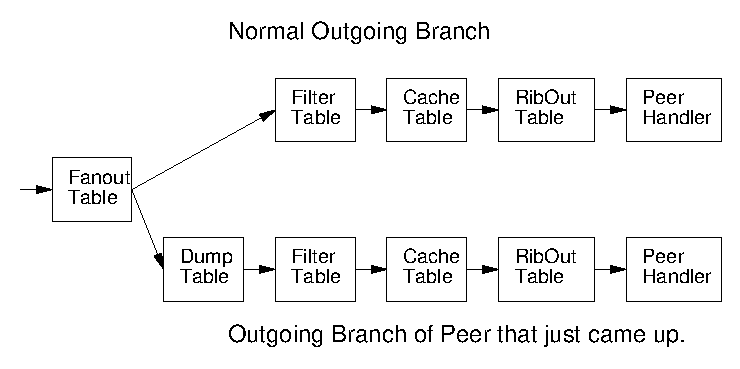
\includegraphics[width=0.6\textwidth]{figs/dump_table}}
\vspace{.05in}
\caption{\label{dump_table}Dynamic insertion of DumpTable on
a peering coming up.}
\end{figure}

A DumpTable is perhaps the most complex part of the BGP machinery.
While the dump is taking place, it must cope with:
\begin{itemize}
\item New routing information being propagated.
\item Other peers going down and coming back, possibly repeatedly.
\end{itemize}
It must do this without propagating inconsistent information downstream,
such as a {\tt replace\_route} or a {\tt delete\_route} without
sending an {\tt add\_route} first.  It must ensure that all the routes
what passed decision are dumped to the new peer. And it must cope when
the routes just before and just after the most recent route it dumped
are deleted, without losing track of where it is in the dump process.

The process is complex enough to merit description here in detail.

Each DumpTable contains a DumpIterator instance which holds all the
state related to the current state of that particular route dump.  The
DumpIterator contains the following state:
\begin{itemize}
\item A list of the remaining peers to dump, initialized at the start
of the dump.  Peers are removed from this list when the dump of the
routes received from that peer is complete, or when the peer does down
during the dump.  Peers are never added to this list during the dump.
\item A list of the peers that went down before we'd finished dumping
them.  Along with each peer is stored enough state to know how far
we'd got though the route dump from that peer before it went down.
\item The current peer whose routes are being dumped.
\item A trie iterator pointing to the next RibIn trie entry to be dumped
on the current peer (we call this the Route Iterator)
\item The last subnet dumped from the current peer.
\item A flag that indicates whether the Route Iterator is currently
valid.
\item The last GenID seen.  The GenID of the RibIn is incremented each
time the peering comes up.
\end{itemize}
At startup the DumpTable initialized the list of remaining peers in
the DumpIterator to be the set of peers that are currently up.  Then
it iterates through this list dumping all the routes from each RibIn
in turn.

The DumpTable calls {\tt dump\_next\_route} on its parent table, passing the
DumpIterator as a parameter.  The {\tt dump\_next\_route} request is relayed
upstream to the DecisionTable.  DecisionTable relays the request to
the input branch of the first peer listed in the list of remaining
peers, and from there it is relayed back to the relevant RibIn.

To allow routes in the RibIn to be deleted during the route dump
without the Route Iterator becoming invalid, we use a special trie and
trie iterator in RibIn, where the route in the trie will not actually
be deleted until no trie iterator is pointing at it.  This is
implemented using reference counts in the Trie nodes themselves.

{\tt dump\_next\_route} in the RibIn checks the Route Iterator to see
if it points to the end of the Trie.  If the previous call to {\tt
dump\_next\_route} had left the Route Iterator pointing to a node that has
subsequently been deleted, this comparison transparently causes the
Route Iterator to move on to the next non-deleted node, or to the end
of the Trie if there are no subsequent deleted nodes.  This updating
of the Route Iterator is transparent to the user of the iterator.

The route pointed to by the Route Iterator is then propated downstream
from the RibIn to the DumpTable as a {\tt route\_dump} call.  The
DumpTable turns this into an {\tt add\_route} call which it propagates
downstream to the new peer.

At the end of {\tt dump\_next\_route}, the RibIn increments the
RouteIterator ready for next time.  

DumpTable then schedules the next call to {\tt dump\_next\_route} using a
zero-second timer to allow other pending events to be processed.

On returning from the timer, the DumpTable checks to see if any route
changes have been queued upstream in the FanoutTable due to output
flow control.  If so, it processes all these route changes before
dumping the next route.  This is necessary, or the DumpTable will not
be able to tell which changes it needs to propagate downstream because
we've already passed their location in the dump process, and which are
unnecessary because we will get round to dumping them eventually.

In general, a route
change needs to be propagated downstream if:
\begin{itemize}
\item It comes from a peer that is not in our remaining peers list.
\item It comes from the peer currently being dumped, but its route is
before the location of the route in the DumpIterator.
\item It comes from a peer that went down, and its subnet is before the
subnet we had reached while dumping that peer's RibIn when the peer
went down.
\item It comes from a peer that went down, and the RibIn GenID later
than that peers GenID was when it went down.  This would happen
because the peering has since come back up, and is now injecting new
routes.
\end{itemize}

When all the routes in the RibIn of a particular peer have been
dumped, that peer is removed from the remaining peers list in the
DumpIterator, and the next {\tt dump\_next\_route} will be sent to the RibIn
of the next peer in the list.

When there are no peers in the remaining peers list, the dump is
complete.  The DumpTable then unplumbs itself from the plumbing, and
deletes itself.

Note that at any time there may be multiple DumpTables in operation,
each dumping to a different peer.  All the dump state is held in the
DumpIterators, so this does not cause any problem.
\end{document}
